\section{Elektrizitätslehre}
\subsection{Elektrischer Stromkreis}
\begin{tabbing}
	\begin{tabu} to \linewidth {l X l X}
		\toprule
		Stromstärke & $I = \frac{\Delta Q}{\Delta t}$ & 
		Widerstand & $R = \frac{U}{I}$ \\
		Ohmsches Gesetz & $U = R \cdot I$ & 
		Widerstand eines Drahtes & R = $\frac{\rho_{el}*l}{A}$ \\
		Elektrische Leistung & $P = UI = \frac{U^2}{R} = I^2 R$ & 
		Elektrische Arbeit & $W = UI\Delta t$ \\
		Stromkosten & $K = W \cdot T$ & \\
		Kapazität Kondensators & $C= \frac{\varepsilon A}{d} \Leftrightarrow Q = CU$ &
		El. Energie Kondensator & $E=\frac{1}{2} CU^2$\\
		Geflossene Ladung & $Q = n * e$ & & \\
	\end{tabu}
\end{tabbing}


\begin{tabbing}
	\begin{tabu} to \linewidth {l X l}
		Variable & Bedeutung & SI-Einheit \\
		\midrule
		$U$ & Spannung& $V$ \\
		$R$ & Widerstand & $\Omega$ \\
		$l$ & Länge des Drahtes & \\
		$\rho_{el}$ & spezifischer Widerstand & \\
		$I$ & Stromstärke & $A$ \\
		$Q$ & geflossene Ladung & $As = C \text{ (couloumb)}$ \\
		$P$ & Leistung & $W$ \\	
		$W$ & Arbeit & $Ws / kwH$ \\
		$T$ & Tarif & $\frac{CHF}{kWh}$ \\
		$K$ & Kosten & $CHF$ \\
		\bottomrule
	\end{tabu}
\end{tabbing}

\begin{tabular}{|l|l|}
Ladung & $q = I t$
\end{tabular}

\subsection{Coulomb Gesetz}
Kraft zwischen zwei Ladungen 

$$ F=\frac{1}{4\pi\epsilon_{0}}\frac{q_{1}q_{2}}{r^2} $$

Gleiche Ladungen stossen sich ab und ungleiche ziehen sich an

\subsection{Elektrisches Feld}

$$ E =\frac{1}{4\pi\epsilon_{0}}\frac{q_{0}}{r^2}\frac{r}{r} $$ todo letzter bruch?
$$ F = qE $$

\subsection{Elektrisches Potential (Potentialunterschied)}

todo

$$ U = R*I $$

\subsection{Widerstand}


$$ R = \frac{l}{\sigma A} = \frac{\rho l}{A} [R]$$

$\sigma$ ist die Leitfähigkeit, $l$ die Länge, $A$ die Fläche des Widerstandes und $\rho$ der spezifische(material) Widerstand.\\
$$\Omega = \frac{V}{A}$$

\subsection{Elektrische Leistung (Verlustleistung)}

Wirkleistung (mechanische Leistung): Die Leistung, die letztendlich genutzt wird. \\
Scheinleistung: Die Leistung, die aus der Messung der Spannung und der Stromstärke errechnet werden kann. \\

$$ P = U*I = R * I^2 $$ 


Leistungsfaktor
$$\frac{P_{W}}{P_{S}} = cos(\phi)$$
mit $\phi$ als Phasenverschiebung

Blindleistung: $P_S*\sin\alpha$

\begin{tabular}{|ll|l|}
Scheinleistung & $S = UI$ & $[P] = VA$ \\
Wirkleistung & $P = UI \cos{\Phi}$ & $[P] = W$ \\
Blindleistung & $Q = UI \sin{\Phi}$ & $[Q] = var$
\end{tabular}



\subsection{Schaltkreise}

\subsubsection{Kirchhoffsche Gesetze}
Die Summe der Ströme in jedem Knoten ist null

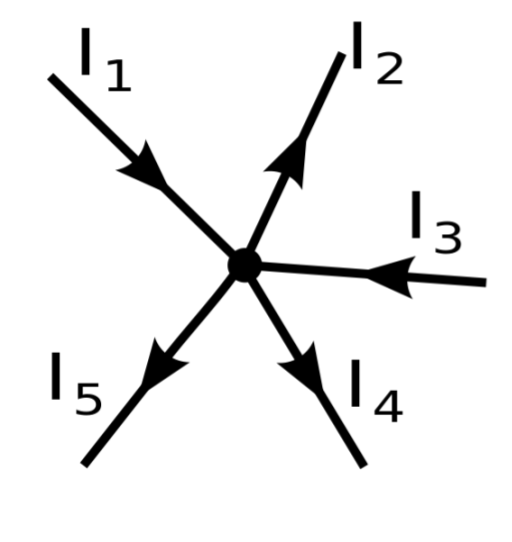
\includegraphics[scale=.3]{images/kirch1.PNG}

$$ \sum I_{k} = 0 $$

Die Summe der Teilspannungen ist null 

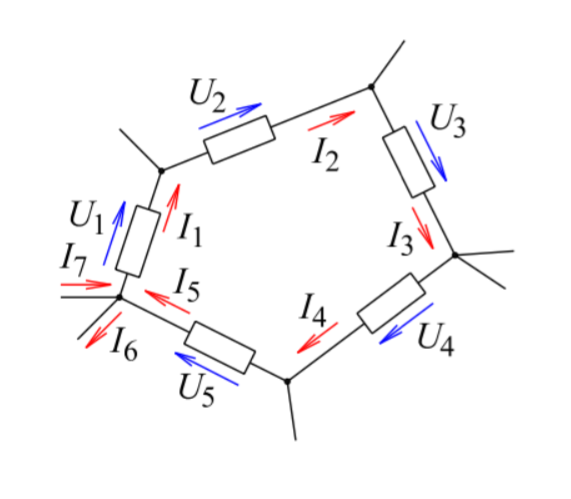
\includegraphics[scale=.3]{images/kirch2.PNG}
$$ \sum U_{k} = 0 $$

\subsubsection{Widerstände}
Reihenschaltung
$$ R_{ges} = R_1 + R_2 + R_3$$
Parallelschaltung
$$ R_{ges} = (\frac{1}{R_1}+\frac{1}{R_2}+\frac{1}{R_3})^{-1} $$



\subsection{Plattenkondensator}


\begin{tabular}{ll}
Kapazität & $  C = \frac{Q}{U} = \frac{\epsilon A}{d} $ \\
Energie & $ E = \frac{1}{2}CU^2 $ \\
Ladung & $Q = \int I(t) dt$ \\
Spannung & $U_C = \frac{\int I(t) dt}{C} = \frac{Q}{C}$
\end{tabular}


\subsection{Magnetfeld}


\begin{tabular}{|ll|l|}
Magnetische Feldstärke & $ H(r) = \frac{1}{2 \pi r} $ & $  = \frac{A}{m}$\\
Magnetische Flussdichte & $ B(r) = \frac{\mu_{0}I}{2\pi r} =  \mu_{0}H$ & $ [B] = 1T = \frac{Vs}{m^2}$ \\
Lorentzkraft (Kraft von Magnetfeld auf Ladung) & $ F = qvB $
\end{tabular}


\subsubsection{Spule}


\begin{tabular}{|ll|l|}
Magnetische Feldstärke & $H = N\frac{I}{l|}$\\
Magnetischer Fluss & $ \Phi = BA $ \\
Induktivität & $ L = N \frac{\Phi}{I} = N^2 \mu_{0} \frac{A}{l|}$ & $[L] = 1H = 1 \frac{Vs}{A}$ \\
& $ A = \pi  (\frac{Durchmesser}{2})^2$ \\
Spannung & $U = L \dot{I}$
\end{tabular}

\subsubsection{Wechselspannung und Wechselstrom}
$$U_{eff} = \frac{U_{max}}{\sqrt{2}}$$
$$I_{eff} = \frac{I_{max}}{\sqrt{2}}$$

\subsubsection{Ohmsches Gesetz der Wechselspannung}
induzierter Blindwiderstand (Spule):
$$R_{L} = \omega L$$ \\
kapazitiver Blindwiderstand (Kondensator):
$$R_{C} = \frac{-1}{\omega C}$$

\subsection{Transformator}
Bei einem Transformator mit einer Primär- und einer Sekundärwicklung, kann man das Verhältnis der Anzahl Windungen der Wicklungen in Relation zum Verhältnis der einzelnen Spannungen setzen.

$$\frac{U_{1}}{U_{2}}=\frac{N_{1}}{N_{2}}$$

dadurch kann man dann z.B. die an der zweiten Wicklung induzierte Spannung berechnen: 

$$U_{2} = U_{1} * \frac{N_{2}}{N_{1}}$$
